\section{Resultados Experimentales}
\subsection{Fotoluminiscencia}
\begin{frame}[t]{System overview}
\frametitle{\secname}
\framesubtitle{\subsecname}
\vspace{-0.5cm}
\begin{tikzpicture}[remember picture, overlay]
\node<1->[anchor = north west, text width =0.67\textwidth, yshift = -0.75cm](txt) at (current page.north west) {
	\begin{tcolorbox}[enhanced,title =\secname,width=\textwidth]
	\begin{itemize}
	\item<1-> Estructuras de Pozos Cuanticos Acoplados
	\item<2-> Fotoluminiscencia (\sm{3171}, \sm{3172} y \sm{3226})
	\item<3-> Fotoluminiscencia (\sm{3140}, \sm{3521} y \sm{3523})
	\end{itemize}
	\end{tcolorbox}	
};

\node<1>[anchor=north west,inner sep=0mm,yshift=10mm,xshift=-3mm] at (txt.north east){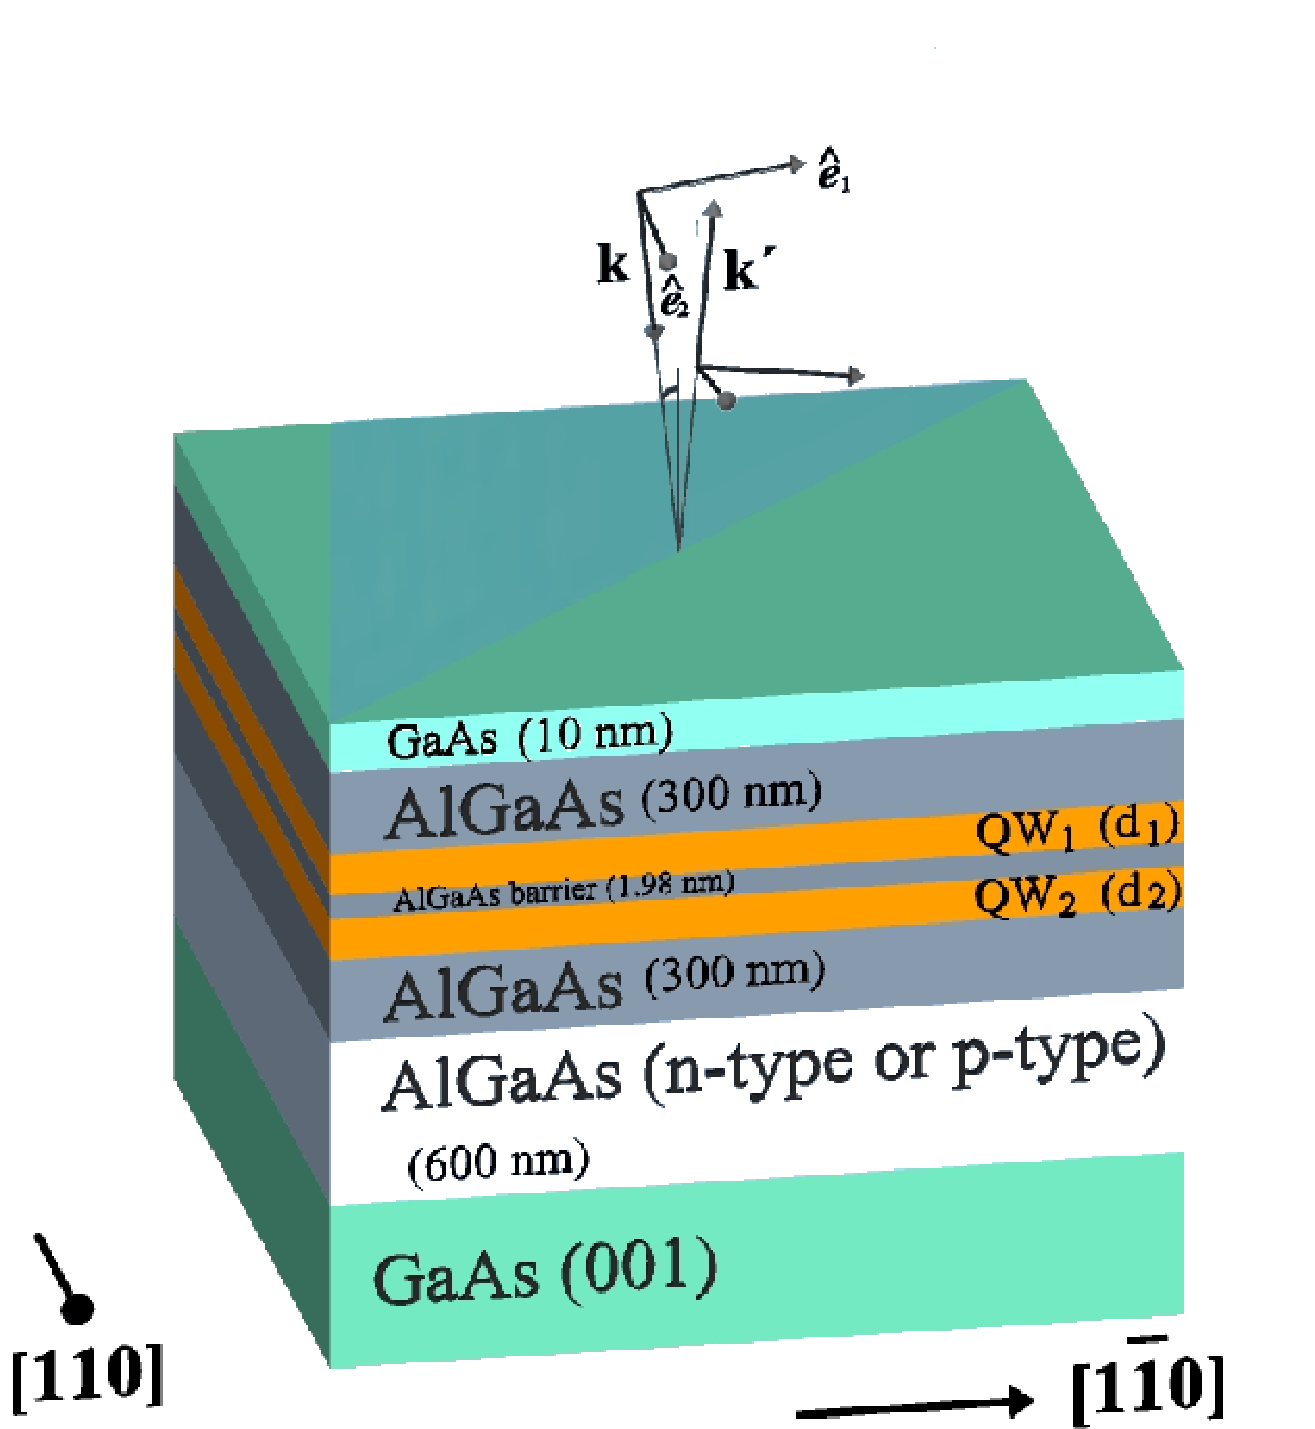
\includegraphics[width=0.4\textwidth]{../beamer-figures/results/Fig_1}};

\node<1>[anchor=south west,inner sep=0mm,yshift=-4mm] at (current page.south west){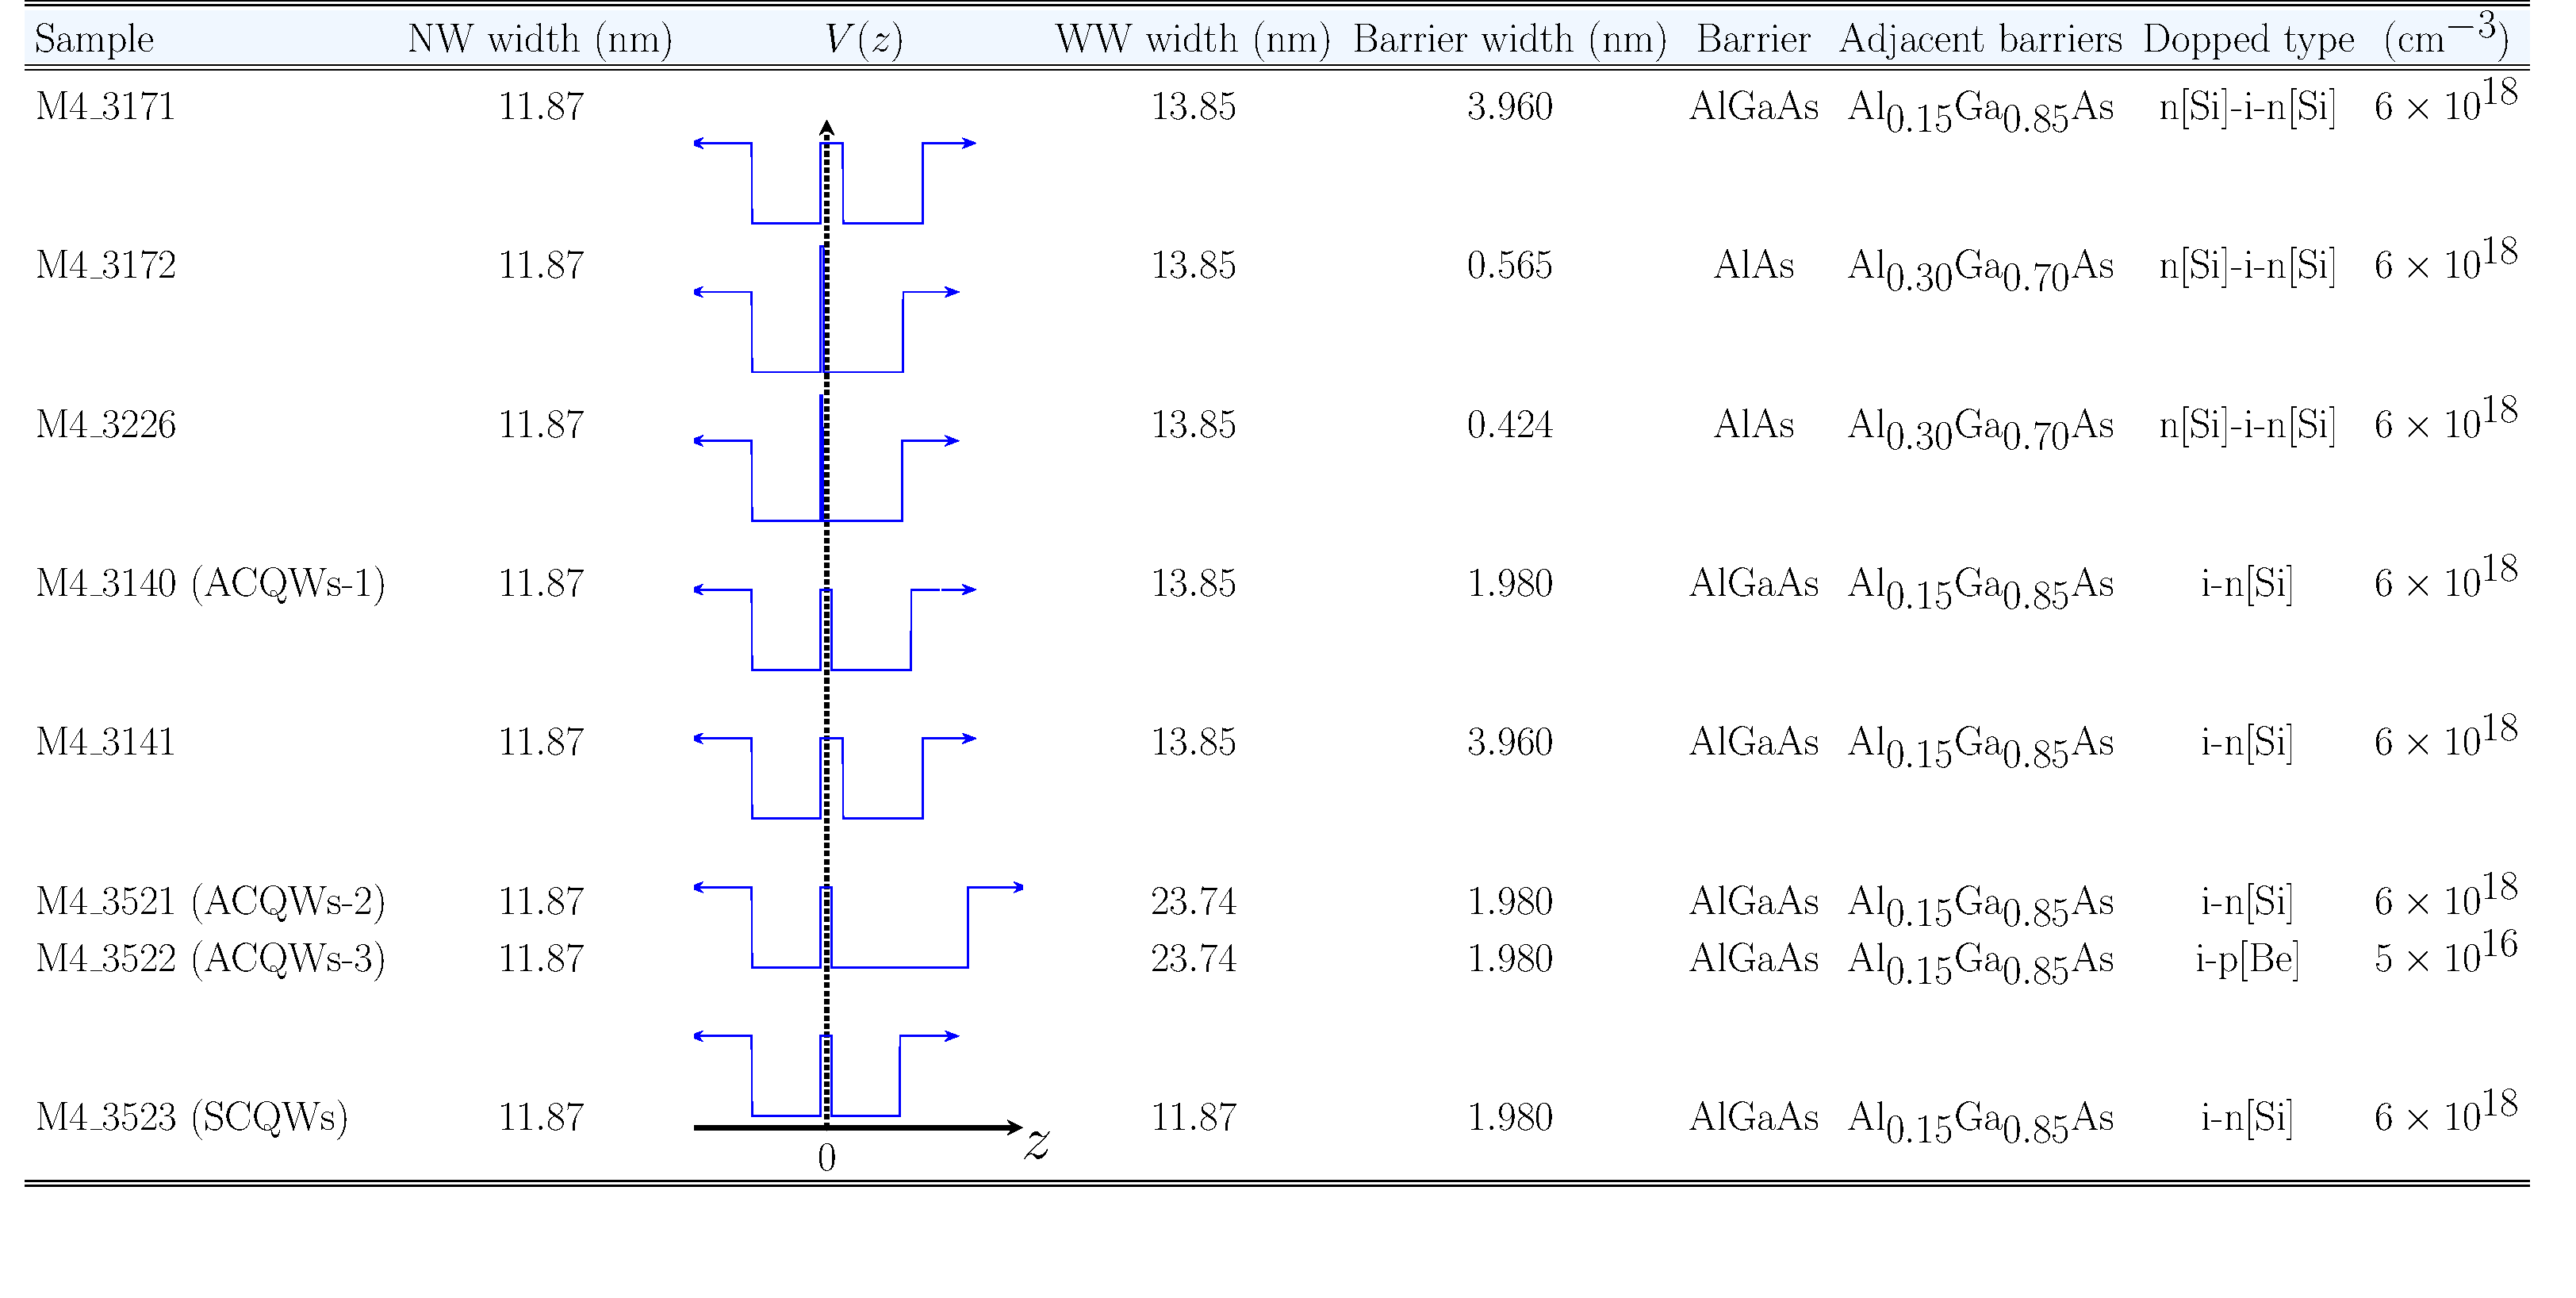
\includegraphics[width=\textwidth]{../../tables/chapter-3/table-1-samples/build-ruco/table-1-samples.pdf}};

\node<2->[anchor=north west,inner sep=0mm,xshift=0mm,yshift=-2mm] at (txt.north east){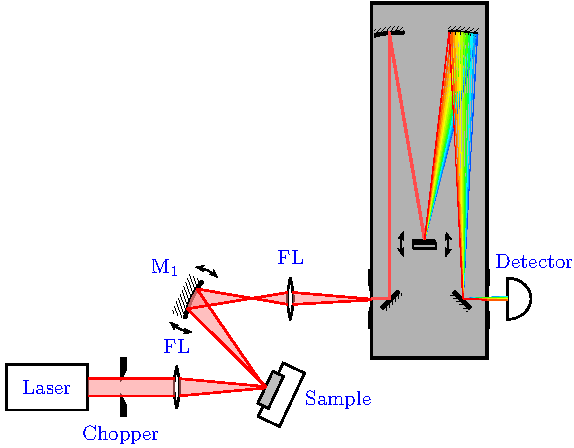
\includegraphics[width=0.33\textwidth]{../../figures/chapter-3/pl-setup/build-ruco/pl-setup}};


\node<2>[anchor=south west,inner sep=0mm,xshift=2mm,yshift=0mm] at (current page.south west){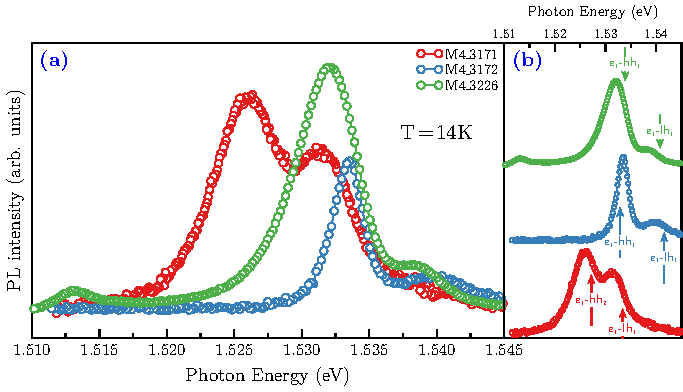
\includegraphics[width=\textwidth]{../../figures/chapter-3/pl-plots/build-ruco/pl-1}};


\node<3>[anchor=south west,inner sep=0mm,xshift=2mm,yshift=0mm] at (current page.south west){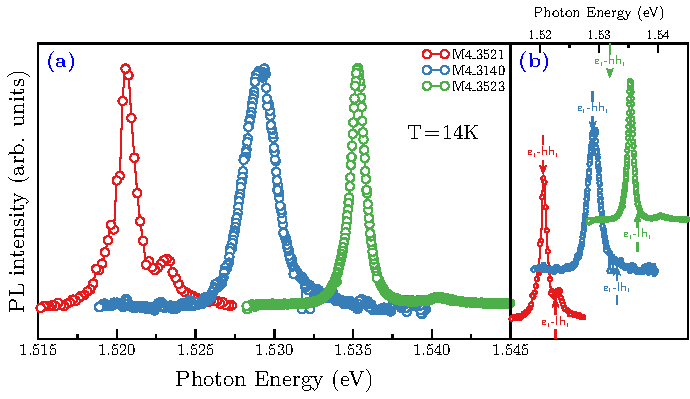
\includegraphics[width=\textwidth]{../../figures/chapter-3/pl-plots/build-ruco/pl-2}};
\end{tikzpicture}
\end{frame}

\subsection{Fotorreflectancia}
\begin{frame}[t]{System overview}
\frametitle{\secname}
\framesubtitle{\subsecname}
\vspace{-0.5cm}
\begin{tikzpicture}[remember picture, overlay]
\node<1->[anchor = north west, text width =0.67\textwidth, yshift = -0.75cm](txt) at (current page.north west) {
	\begin{tcolorbox}[enhanced,title =\secname,width=\textwidth]
	\begin{itemize}
	\item<1-> Fotorreflectancia (\sm{3171}, \sm{3172} y \sm{3226})
	\item<2-> Fotorreflectancia (\sm{3140}, \sm{3521} y \sm{3523})
	\item<3-> Efectos Excitonicos
	\end{itemize}
	\end{tcolorbox}	
};



% \node<1>[anchor=south west,inner sep=0mm,yshift=5mm] at (current page.south west){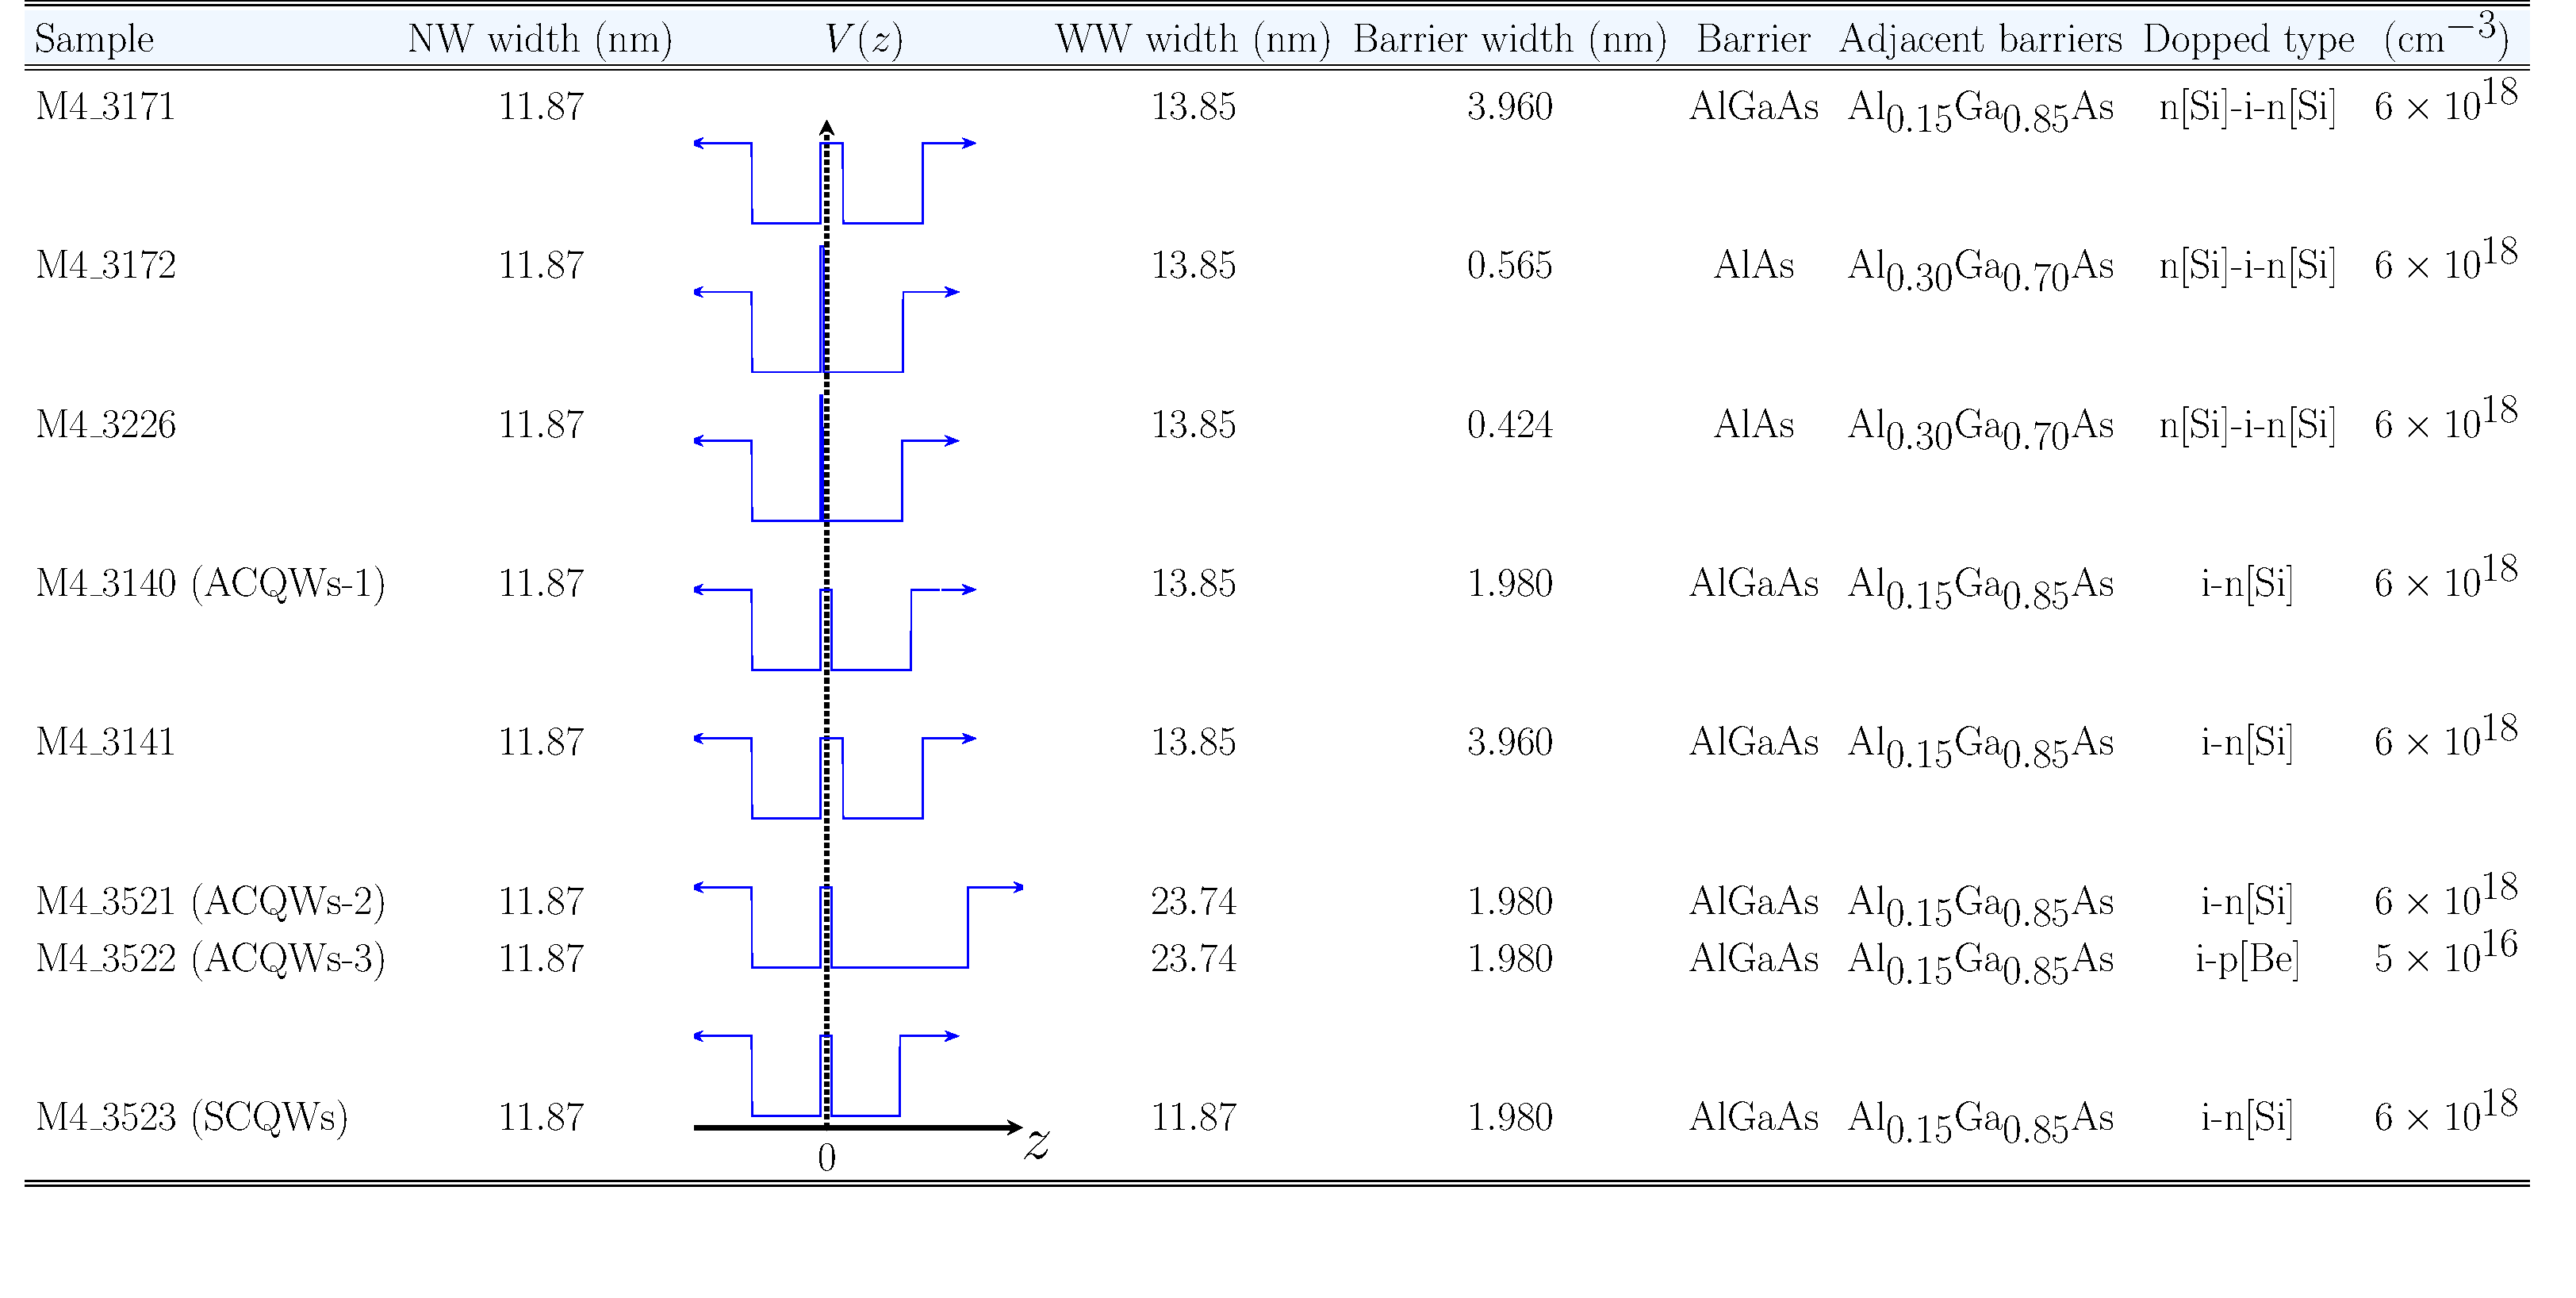
\includegraphics[width=1.045\textwidth]{../../tables/chapter-3/table-1-samples/build-ruco/table-1-samples.pdf}};

\node<1->[anchor=north west,inner sep=0mm,xshift=0mm,yshift=-2mm] at (txt.north east){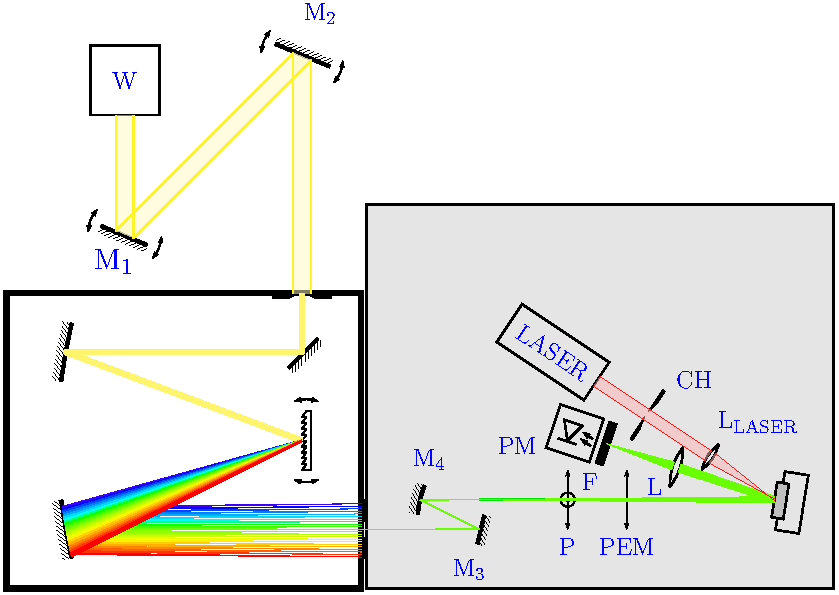
\includegraphics[width=0.33\textwidth]{../../figures/chapter-3/pr-setup/build-ruco/pr-setup}};


\node<1>[anchor=south west,inner sep=0mm,xshift=2mm,yshift=0mm] at (current page.south west){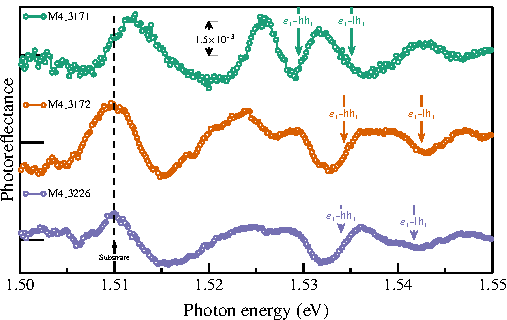
\includegraphics[width=0.95\textwidth]{../../figures/chapter-3/pr-plots/build-ruco/pr-set1.pdf}};
\node<2>[anchor=south west,inner sep=0mm,xshift=2mm,yshift=0mm] at (current page.south west){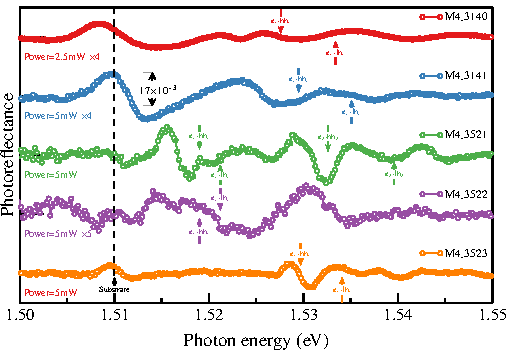
\includegraphics[width=0.87\textwidth]{../../figures/chapter-3/pr-plots/build-ruco/pr-set2.pdf}};
\node<3>[anchor=south west,inner sep=0mm,xshift=2mm,yshift=0mm] at (current page.south west){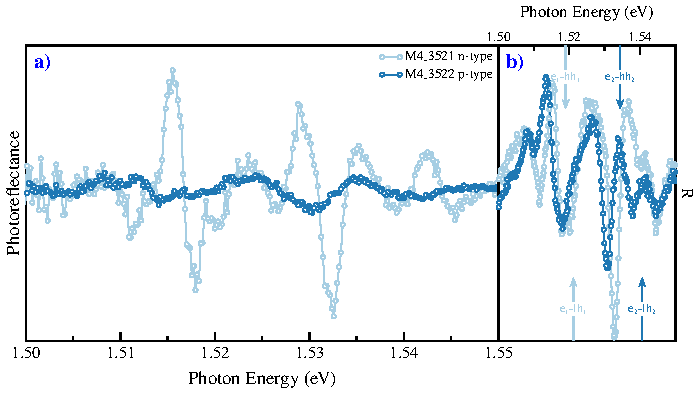
\includegraphics[width=\textwidth]{../../figures/chapter-3/pr-plots/build-ruco/pr-set3.pdf}};
\node<4>[anchor=south west,inner sep=0mm,xshift=2mm,yshift=0mm] at (current page.south west){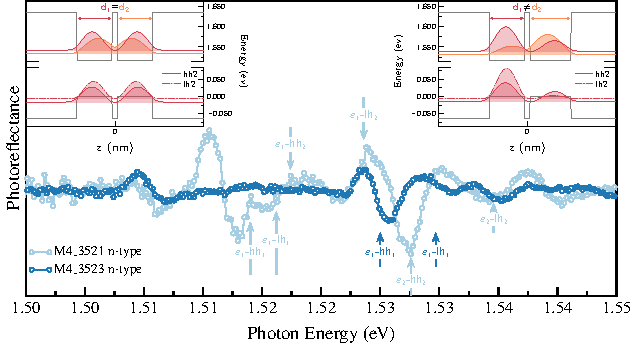
\includegraphics[width=0.85\textwidth]{../../figures/chapter-3/pr-plots/build-ruco/pr-set4.pdf}};
\node<5>[anchor=south west,inner sep=0mm,xshift=2mm,yshift=0mm] at (current page.south west){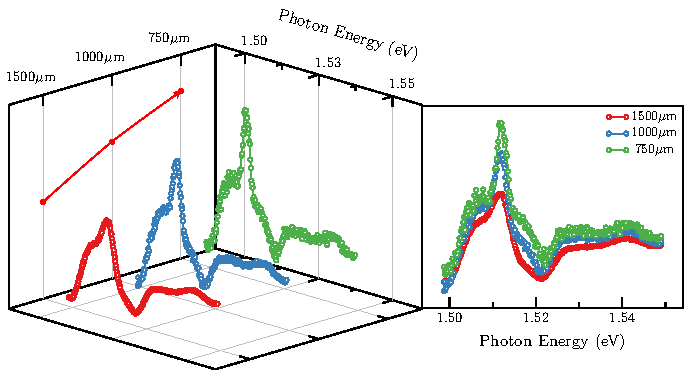
\includegraphics[width=\textwidth]{../../figures/chapter-3/pr-plots/build-ruco/pr-set5.pdf}};
\node<6>[anchor=south west,inner sep=0mm,xshift=2mm,yshift=0mm] at (current page.south west){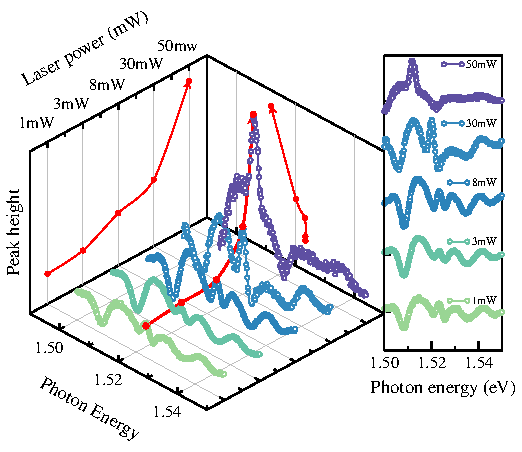
\includegraphics[width=0.75\textwidth]{../../figures/chapter-3/pr-plots/build-ruco/pr-set6.pdf}};

\node<7->[anchor=south west,inner sep=0mm,xshift=0mm,yshift=0mm](t1) at (current page.south west){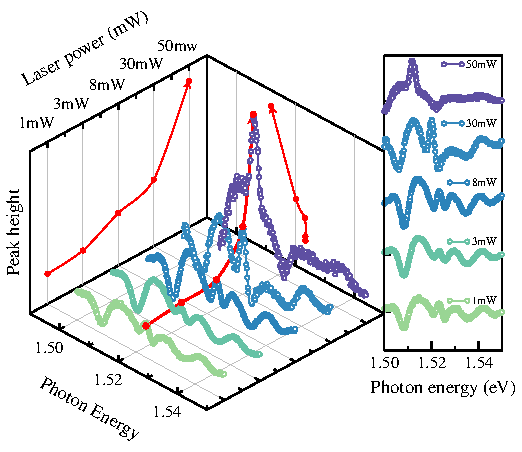
\includegraphics[width=0.3\textwidth]{../../figures/chapter-3/pr-plots/build-ruco/pr-set6.pdf}};

\node<7>[anchor=north west,inner sep=0mm,xshift=20mm,yshift=-5mm] at (txt.south west){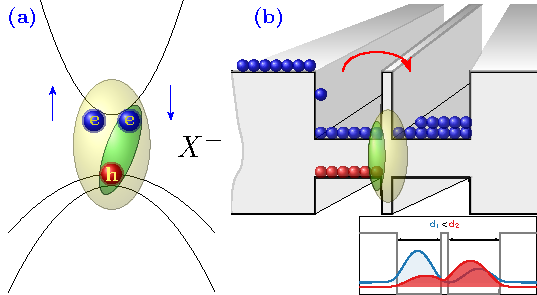
\includegraphics[width=0.8\textwidth]{../../figures/chapter-3/trions-scheme/build-ruco/trions-sheme}};

\node<8>[anchor=south east,inner sep=0mm,xshift=-22mm,yshift=0mm] at (current page.south east){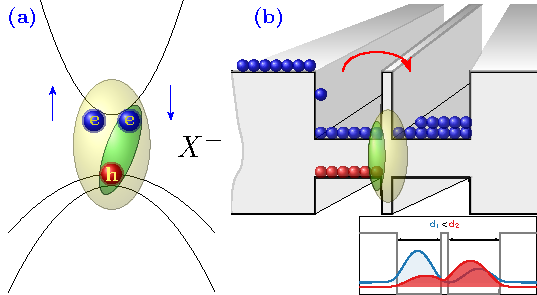
\includegraphics[width=0.45\textwidth]{../../figures/chapter-3/trions-scheme/build-ruco/trions-sheme}};


\node<8>[anchor=north west,inner sep=0mm,xshift=0mm,yshift=-2mm] at (txt.south west){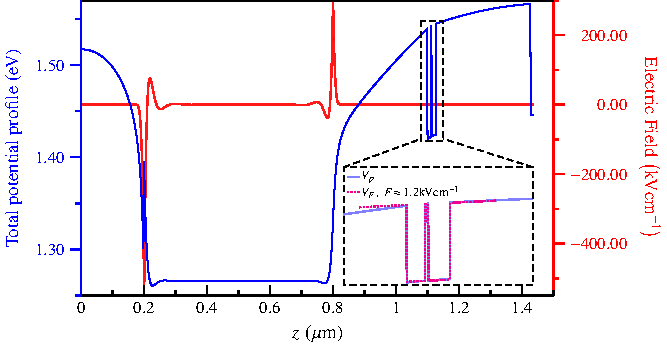
\includegraphics[width=0.8\textwidth]{../../figures/chapter-3/poisson/build/poisson-3.pdf}};
% \node<3>[anchor=south west,inner sep=0mm,xshift=2mm,yshift=0mm] at (current page.south west){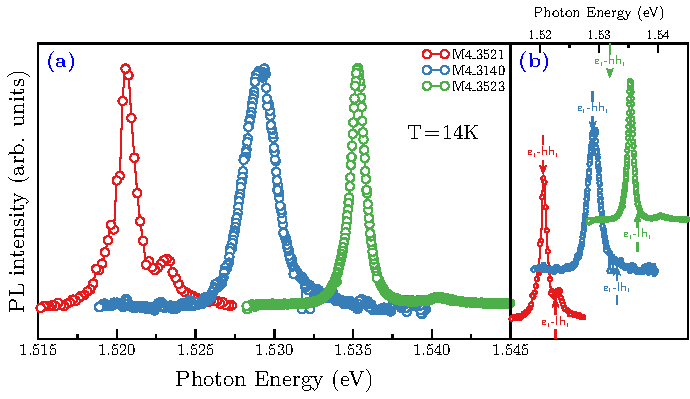
\includegraphics[width=\textwidth]{../../figures/chapter-3/pl-plots/build-ruco/pl-2}};
\end{tikzpicture}
\end{frame}
	

\subsection{Reflectancia Diferencial}
\begin{frame}[t]{System overview}
\frametitle{\secname}
\framesubtitle{\subsecname}
\vspace{-0.5cm}
\begin{tikzpicture}[remember picture, overlay]
\node<1->[anchor = north east, text width =0.37\textwidth, yshift = -7mm,xshift=-20mm](txt) at (current page.north east) {
	\begin{tcolorbox}[enhanced,title =\secname,width=\textwidth]
	\begin{itemize}
	\item<1-> RAS set 1
	\item<2-> RAS set 2
	\item<3-> Asimmetria$\rightarrow C_{2v}$
	\end{itemize}
	\end{tcolorbox}	
};



% \node<1>[anchor=south west,inner sep=0mm,yshift=5mm] at (current page.south west){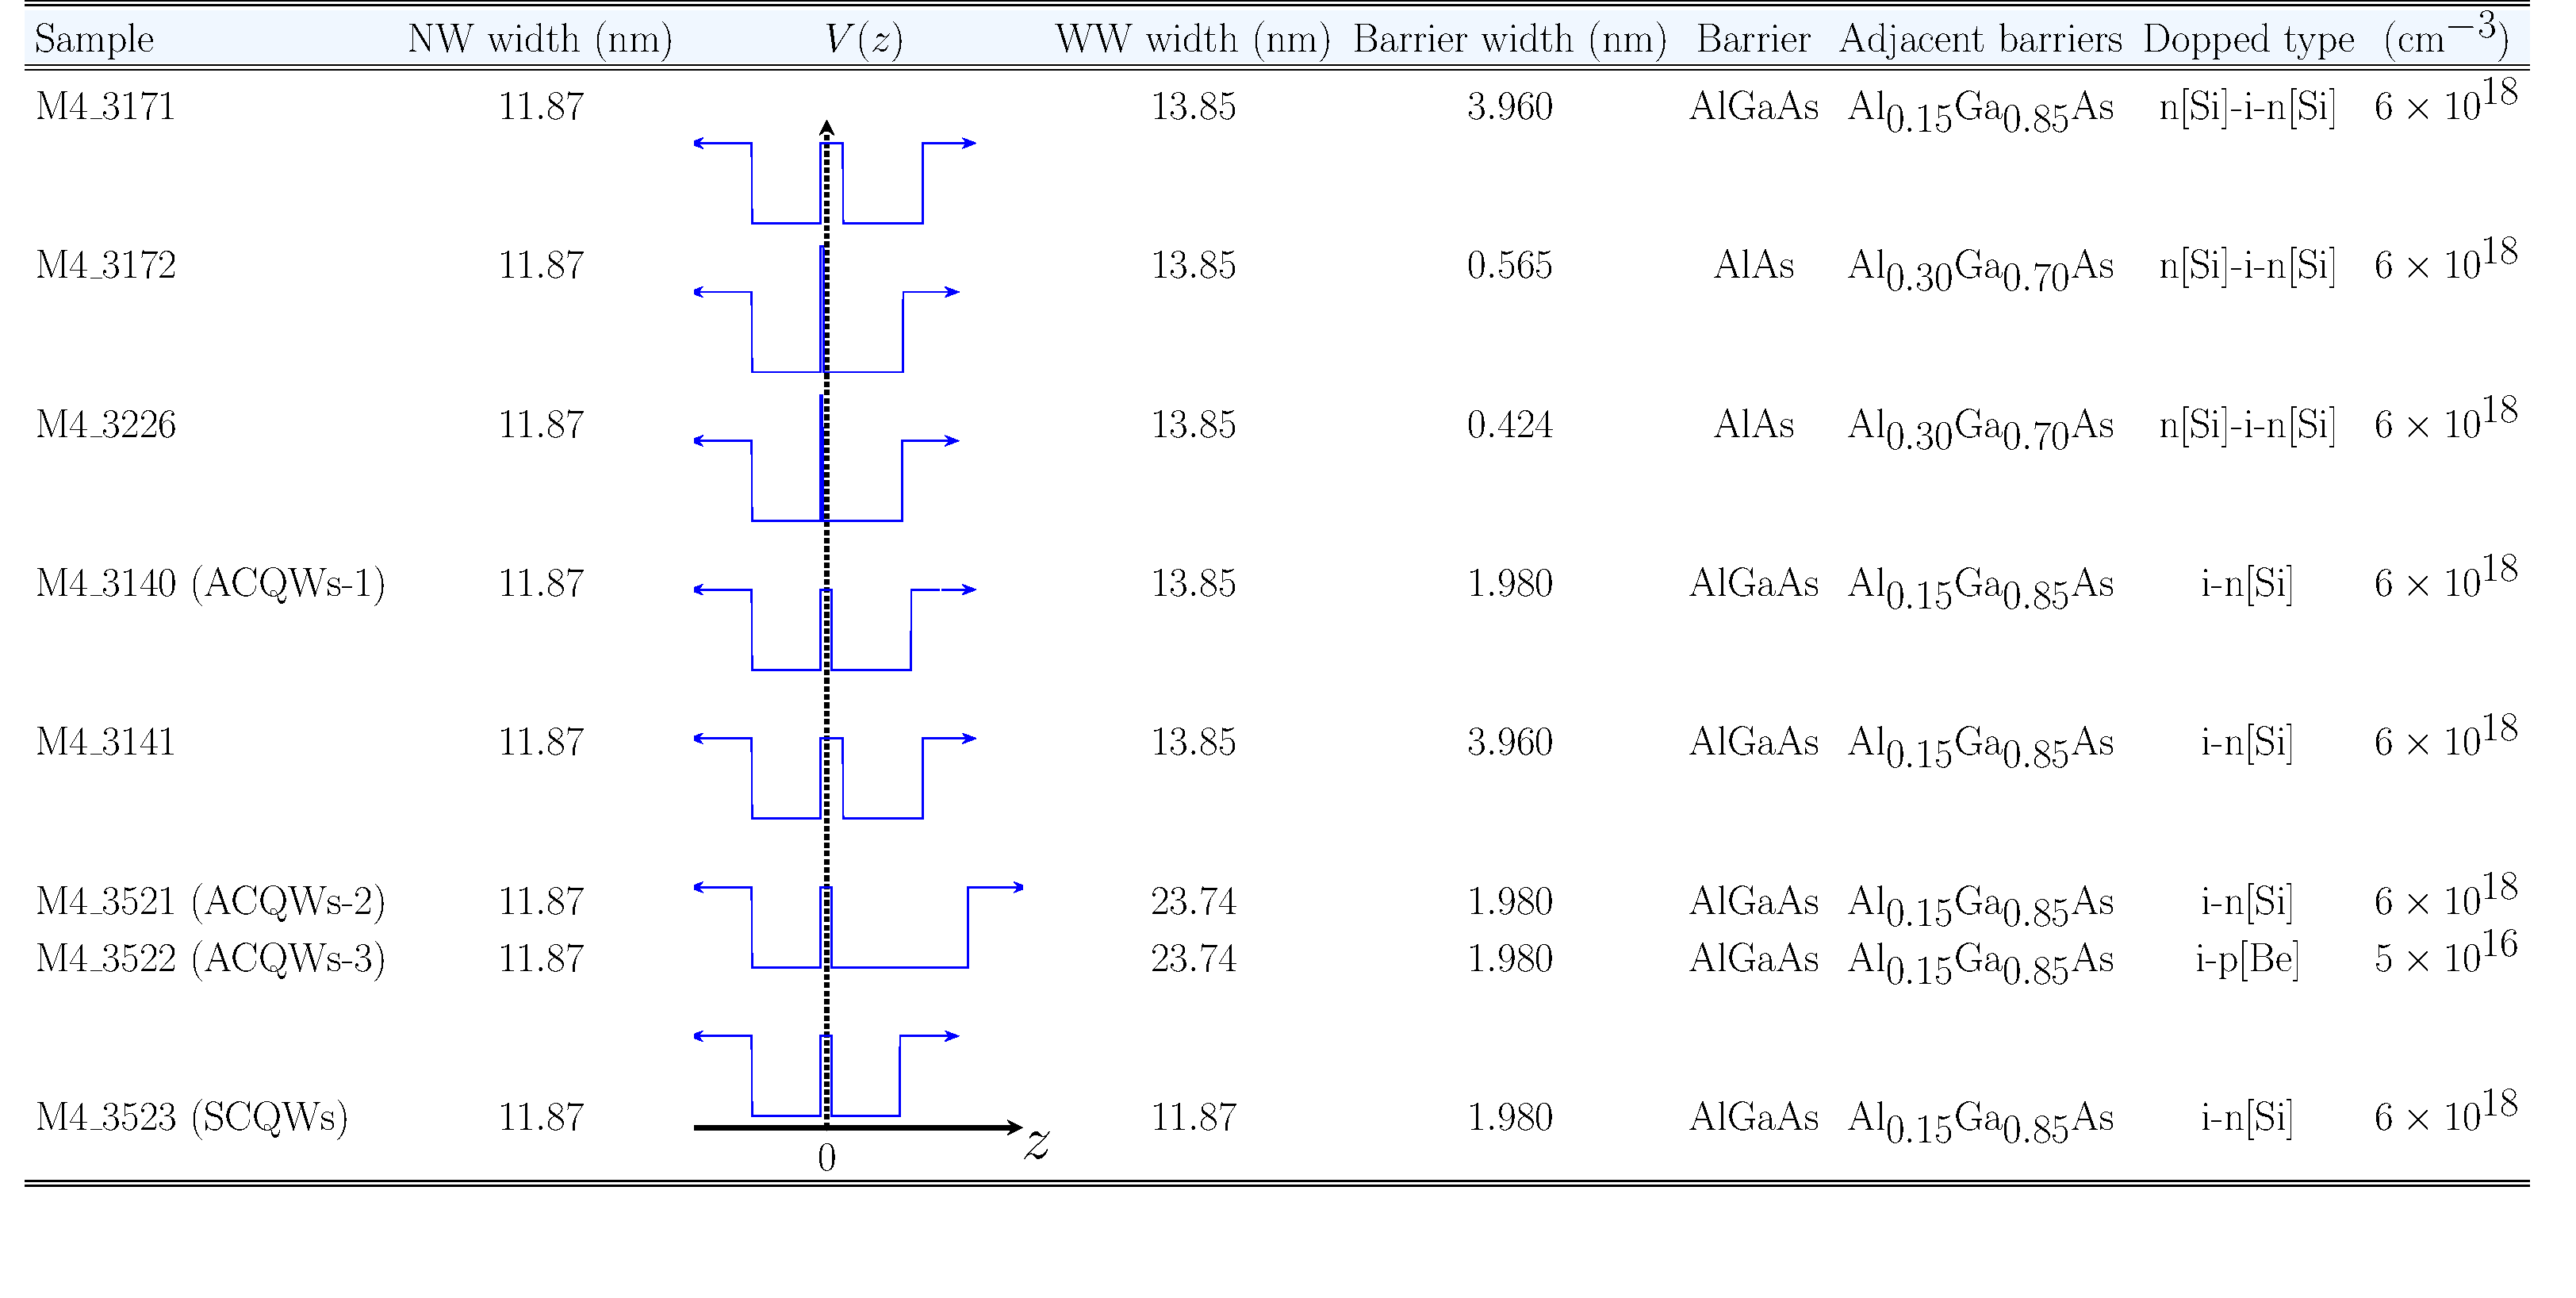
\includegraphics[width=1.045\textwidth]{../../tables/chapter-3/table-1-samples/build-ruco/table-1-samples.pdf}};

\node<1-2>[anchor=south east,inner sep=0mm,xshift=-20mm,yshift=0mm] at (current page.south east){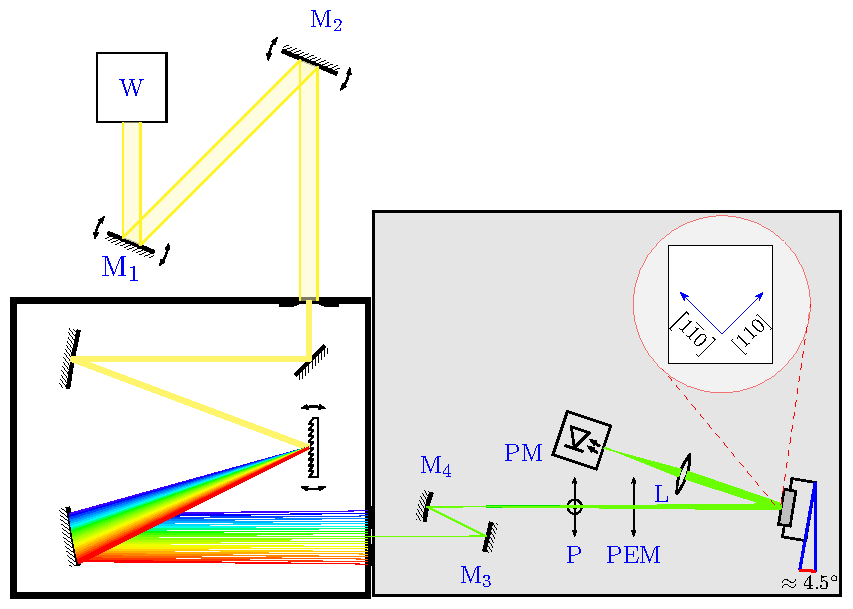
\includegraphics[width=0.38\textwidth]{../../figures/chapter-3/ras-setup/build-ruco/ras-setup-2}};


\node<1>[anchor=north west,inner sep=0mm,xshift=-1mm,yshift=-10mm] at (current page.north west){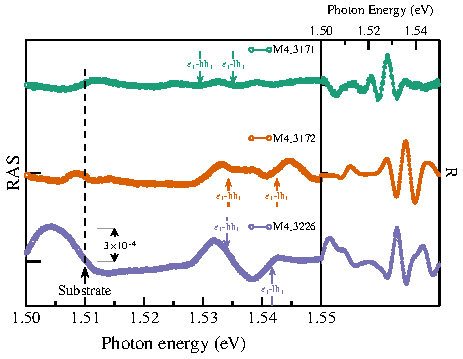
\includegraphics[width=0.7\textwidth]{../../figures/chapter-3/ras-plots/build-ruco/ras-set-1.pdf}};
\node<2>[anchor=north west,inner sep=0mm,xshift=-1mm,yshift=-10mm] at (current page.north west){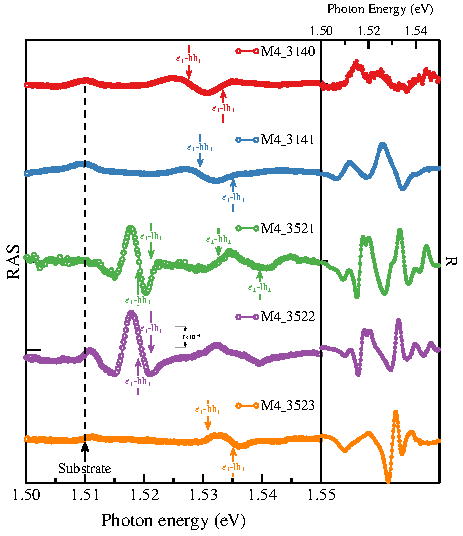
\includegraphics[width=0.7\textwidth]{../../figures/chapter-3/ras-plots/build-ruco/ras-set-2.pdf}};
\node<3-5>[anchor=north west,inner sep=0mm,xshift=-1mm,yshift=-10mm] at (current page.north west){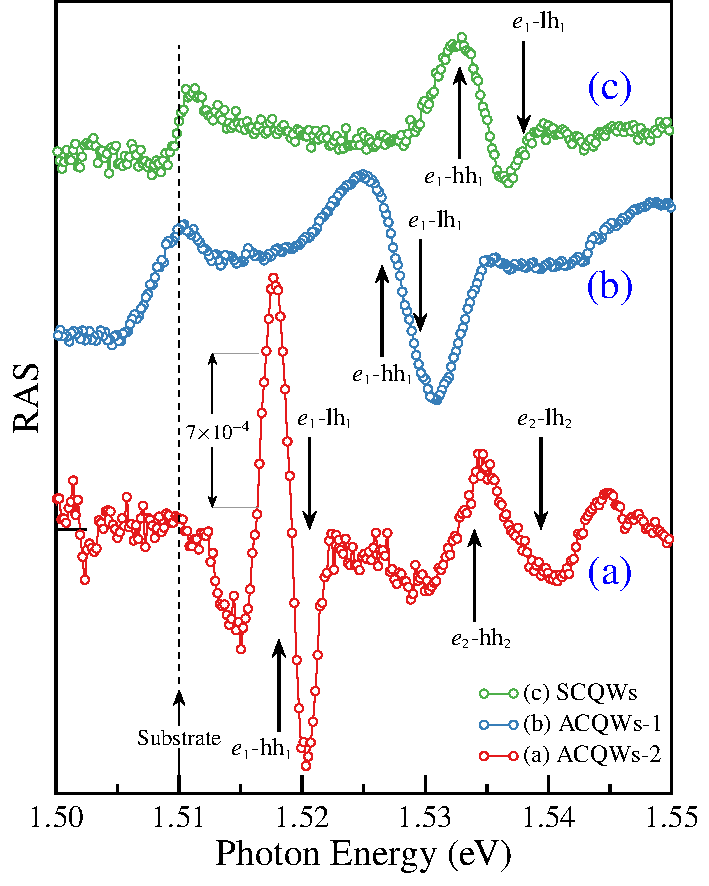
\includegraphics[width=0.65\textwidth]{../../figures/chapter-3/ras-plots/build-ruco/ras-set-3.pdf}};

\node<6>[anchor=north west,inner sep=0mm,xshift=-1mm,yshift=-10mm] at (current page.north west){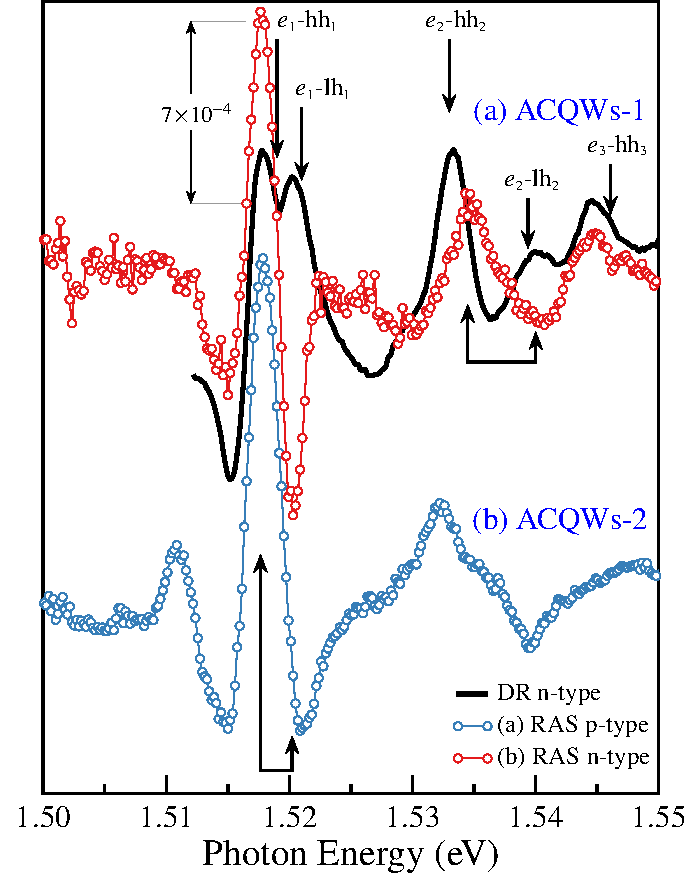
\includegraphics[width=0.65\textwidth]{../../figures/chapter-3/ras-plots/build-ruco/ras-set-4.pdf}};

\node<7>[anchor=north west,inner sep=0mm,xshift=-1mm,yshift=-10mm] at (current page.north west){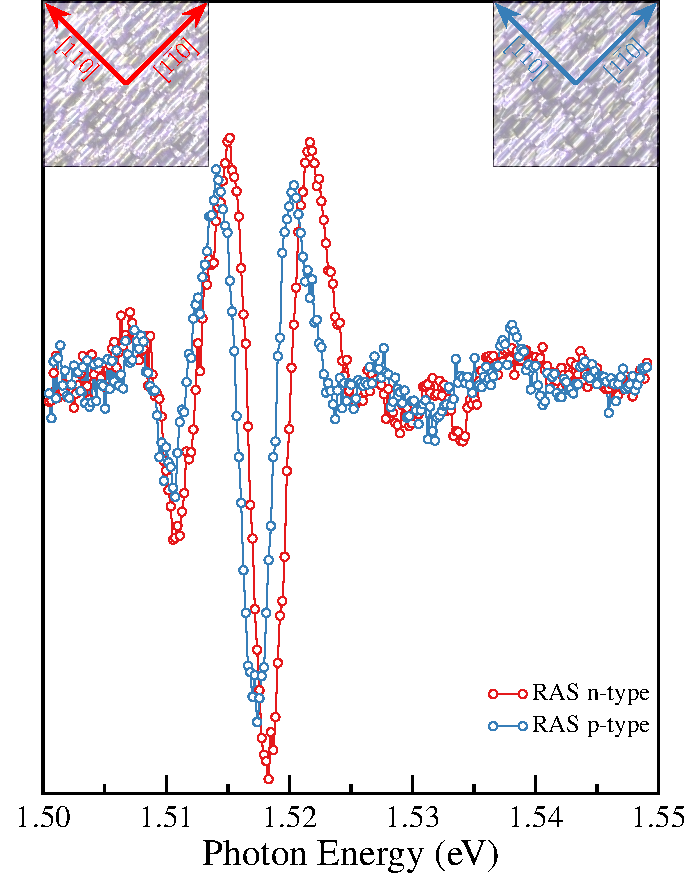
\includegraphics[width=0.65\textwidth]{../../figures/chapter-3/ras-plots/build-ruco/ras-set-5.pdf}};

\node<4->[anchor=north west,text width=0.37\textwidth,scale=0.8,xshift=-3mm](e1) at (txt.south west){
	\begin{equation*}
		\dfrac{
		   \braket{\psi_{\mathrm{en}}} {\psi_{\mathrm{hhn}}}
		   \mel{\psi_{\mathrm{hhn}}}{\cal{H}}{\psi_{\mathrm{lhn}}}
		   \braket{\psi_{\mathrm{lhn}}} {\psi_{\mathrm{en}}}
		  }
		  {\mathrm{\Delta E_{n}}
		  }
	\end{equation*}
};

\node<4>[anchor=north,text width=0.3\textwidth,scale=0.9,xshift=4mm] at (e1.south){
	\begin{equation*}
		\mathrm{\Delta E_{n} = E_{hhn} - E_{lhn}}
	\end{equation*}
};

\node<5->[anchor=south east,inner sep=0mm,xshift=-21mm,yshift=0mm] at (current page.south east){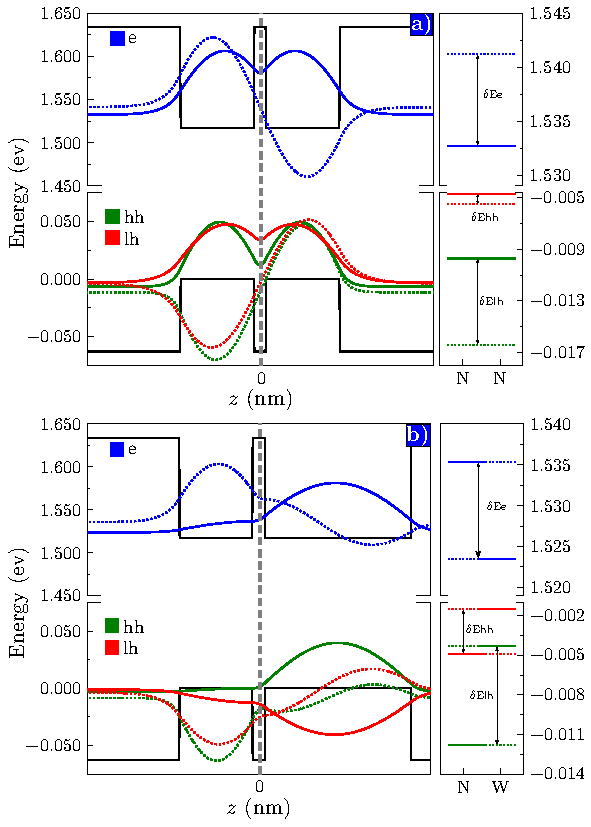
\includegraphics[width=0.4\textwidth]{../../figures/chapter-2/numerical-calculations/out/numerical-results-model.pdf}};

\end{tikzpicture}
\end{frame}
	